%!TEX program = xelatex
\documentclass[dvipsnames, svgnames,a4paper,11pt]{article}
% ----------------------------------------------------- 
%	加边框的命令
%	参考:https://tex.stackexchange.com/questions/531559/how-to-add-the-page-border-for-first-two-pages-in-latex
\usepackage{tikz}
\usetikzlibrary{calc}
\usepackage{eso-pic}
\AddToShipoutPictureBG{%
\begin{tikzpicture}[overlay,remember picture]
\draw[line width=0.6pt] % 边框粗细
    ($ (current page.north west) + (0.6cm,-0.6cm) $)
    rectangle
    ($ (current page.south east) + (-0.6cm,0.6cm) $); % 边框位置
\end{tikzpicture}}


\usepackage{xcolor}
\definecolor{c1}{HTML}{070F94} % 目录颜色 原版为2752C9 紫灰色535AAA 蓝紫色0B0DB7 深蓝色070F94 湖绿色219394 松石灰绿086173
\definecolor{c2}{HTML}{E20129} % 引用颜色 原版\definecolor{c2}{RGB}{190,20,83} 橙色F24729

\usepackage{ctex}
\usepackage[top=28mm,bottom=28mm,left=15mm,right=15mm]{geometry}
\usepackage{hyperref} 
\hypersetup{
	colorlinks,
	linktoc = section, % 超链接位置,选项有section, page, all
	linkcolor = c1, % linkcolor 目录颜色
	citecolor = c1  % citecolor 引用颜色
}
\usepackage{amsmath,enumerate,multirow,float}
\usepackage{tabularx}
\usepackage{tabu}
\usepackage{subfig}
\usepackage{fancyhdr}
\usepackage{graphicx}
\usepackage{wrapfig}  
\usepackage{physics}
\usepackage{appendix}
\usepackage{amsfonts}

%
\usepackage{tcolorbox}
\tcbuselibrary{skins,breakable}
\newtcolorbox{tbox}[2][]{
    colframe=black!70!,
    breakable,
    enhanced,
	boxrule =0.5pt,
    title = {#2},
    fonttitle = \large\kaishu\bfseries,
	drop fuzzy shadow,
    #1
}
\newtcolorbox[auto counter,number within=section]{question}[1][]{
  top=2pt,bottom=2pt,arc=1mm,
  boxrule=0.5pt,
%   frame hidden,
  breakable,
  enhanced, %跨页后不会显示下边框
  coltitle=c1!80!gray,
  colframe=c1,
  colback=c1!3!white,
  drop fuzzy shadow,
  title={思考题~\thetcbcounter:\quad},
  fonttitle=\bfseries,
  attach title to upper,
  #1
}

% ---------------------------------------------------------------------
%	利用cleveref改变引用格式,\cref是引用命令
\usepackage{cleveref}
\crefformat{figure}{#2{\textcolor{c2}{Figure #1}}#3} % 图片的引用格式
\crefformat{equation}{#2{(\textcolor{c2}{#1})}#3} % 公式的引用格式
\crefformat{table}{#2{\textcolor{c2}{Table #1}}#3} % 表格的引用格式


% ---------------------------------------------------------------------
%	页眉页脚设置
\fancypagestyle{plain}{\pagestyle{fancy}}
\pagestyle{fancy}
\lhead{\kaishu 中山大学物理与天文学院基础物理实验\uppercase\expandafter{\romannumeral2}} % 左边页眉,学院 + 课程
\rhead{\kaishu 实验报告By黄罗琳} % 右边页眉,实验报告标题
\cfoot{\thepage} % 页脚,中间添加页码


% ---------------------------------------------------------------------
%	对目录、章节标题的设置
\renewcommand{\contentsname}{\centerline{\huge 目录}}
\usepackage{titlesec}
\usepackage{titletoc}
% \titleformat{章节}[形状]{格式}{标题序号}{序号与标题间距}{标题前命令}[标题后命令]
\titleformat{\section}{\centering\LARGE\songti}{}{1em}{}

% ---------------------------------------------------------------------
%   listing代码环境设置
\usepackage{listings}
\lstloadlanguages{python}
\lstdefinestyle{pythonstyle}{
backgroundcolor=\color{gray!5},
language=python,
frameround=tftt,
frame=shadowbox, 
keepspaces=true,
breaklines,
columns=spaceflexible,                   
basicstyle=\ttfamily\small, % 基本文本设置,字体为teletype,大小为scriptsize
keywordstyle=[1]\color{c1}\bfseries, 
keywordstyle=[2]\color{Red!70!black},   
stringstyle=\color{Purple},       
showstringspaces=false,
commentstyle=\ttfamily\scriptsize\color{green!40!black},%注释文本设置,字体为sf,大小为smaller
tabsize=2,
morekeywords={as},
morekeywords=[2]{np, plt, sp},
numbers=left, % 代码行数
numberstyle=\it\tiny\color{gray}, % 代码行数的数字字体设置
stepnumber=1,
rulesepcolor=\color{gray!30!white}
}




% ---------------------------------------------------------------------
%	其他设置
\def\degree{${}^{\circ}$} % 角度
\graphicspath{{./images/}} % 插入图片的相对路径
\allowdisplaybreaks[4]  %允许公式跨页 
\usepackage{lipsum}
\usepackage{adjustbox}
\usepackage{lipsum}
\usepackage{enumitem}
\usepackage{tabularray}
%\usepackage{mathrsfs} % 字体
%\captionsetup[figure]{name=Figure} % 图片形式
%\captionsetup[table]{name=Table} % 表格形式
\begin{document}
	
	% 实验报告封面	
	% 顶栏
	\begin{table}
		\renewcommand\arraystretch{1.7}
		\begin{tabularx}{\textwidth}{
				|X|X|X|X
				|X|X|X|X|}
			\hline
			\multicolumn{2}{|c|}{预习报告}&\multicolumn{2}{|c|}{实验记录}&\multicolumn{2}{|c|}{分析讨论}&\multicolumn{2}{|c|}{总成绩}\\
			\hline
			\LARGE25 & & \LARGE25 & & \LARGE30 & & \LARGE80 & \\
			\hline
		\end{tabularx}
	\end{table}
	% ---
	
	% 信息栏
	\begin{table}
		\renewcommand\arraystretch{1.7}
		\begin{tabularx}{\textwidth}{|X|X|X|X|}
			\hline
			年级、专业: & 2022级 物理学 &组号: &实验组1 \\
			\hline
			姓名: &   黄罗琳 & 学号: &  22344001 \\
			\hline
			实验时间: & 2024/4/17 & 教师签名: & \\
			\hline
		\end{tabularx}
	\end{table}
	% ---
	
	% 大标题
	\begin{center}
		\LARGE CA3 \quad 原子的发射和吸收光谱观测分析实验
	\end{center}
	
	\textbf{【实验报告注意事项】}
	\begin{enumerate}
		
		\item 实验报告由三部分组成:
	\begin{enumerate}[label=\textup{(\arabic*)}]
		\item 预习报告:课前认真研读\underline{\textbf{实验讲义}},实验所需的仪器设备、用具及其使用、完成课前预习思考题;了解实验需要测量的物理量,并根据要求提前准备实验记录表格(可以参考实验报告模板,可以打印)。\textcolor{red}{\textbf{(25分)}}
		
	    \item 实验记录:认真、客观记录实验条件、实验过程中的现象以及数据。实验记录请用珠笔或者钢笔书写并签名(\textcolor{red}{\textbf{用铅笔记录的被认为无效}})。\textcolor{red}{\textbf{保持原始记录,包括写错删除部分,如因误记需要修改记录,必须按规范修改。}}(不得输入电脑打印,但可扫描手记后打印扫描件);离开前请实验教师检查记录并签名。\textcolor{red}{\textbf{(30分)}}
	    
	    \item 数据处理及分析讨论:处理实验原始数据(学习仪器使用类型的实验除外),对数据的可靠性和合理性进行分析;按规范呈现数据和结果(图、表),包括数据、图表按顺序编号及其引用;分析物理现象(含回答实验思考题,写出问题思考过程,必要时按规范引用数据);最后得出结论。\textcolor{red}{\textbf{(25分)}}
	    
	\end{enumerate}
	\textbf{实验报告就是将预习报告、实验记录、和数据处理与分析合起来,加上本页封面。}
	\item 每次完成实验后的一周内交\textbf{实验报告}(特殊情况不能超过两周)。
	\item 注意事项:
		\begin{enumerate}[label=\textup{(\arabic*)}]
			\item 实验中\textcolor{red}{\textbf{光纤不能过度弯折}};
			\item 信号强度不能过饱和值;
			\item 光源长时间通电后会\textcolor{red}{\textbf{发热}},小心烫手,切换光源时务必注意(可等断电冷却后再碰);
			\item \textcolor{red}{\textbf{请提前了解光纤光谱仪的基本工作原理与关键参数等。}}
		\end{enumerate}
\end{enumerate}

	
	
	\clearpage
	\tableofcontents
	\clearpage
	
	\setcounter{section}{0}
	\section{CA3 \quad 原子的发射和吸收光谱观测分析实验 \quad\heiti 预习报告}
		
	\subsection{实验目的}
		\begin{enumerate}
			\item 原子发射光谱的观测:
				\begin{enumerate}
					\item 学习光纤光谱仪的使用;
					\item 观测钠原子光谱,了解碱金属原子光谱的一般规律;
					\item 观测汞原子光谱,了解中外层电子与原子核相互作用;
					\item 观测多种光源的发射光谱,了解线光谱与连续谱的异同。
				\end{enumerate}
			\item  原子吸收光谱的观测:
				\begin{enumerate}
					\item 调配不同浓度的高锰酸钾水溶液;
					\item 测量高锰酸钾水溶液的紫外-可见吸收光谱,找出吸收峰;
					\item 测量不同浓度高锰酸钾水溶液的紫外-可见吸收光谱,验证比尔定律;
					\item 测量不同片数玻璃基板的透过光谱,验证朗伯定律。
				\end{enumerate}
		\end{enumerate}
		
	
	\subsection{仪器用具}
		\begin{table}[htbp]
			\centering
			\renewcommand\arraystretch{1.6}
			% \setlength{\tabcolsep}{10mm}
			\begin{tabular}{p{0.05\textwidth}|p{0.20\textwidth}|p{0.05\textwidth}|p{0.5\textwidth}}
			\hline
			编号& 仪器用具名称 & 数量 &  主要参数(型号,测量范围,测量精度等) \\
			\hline
			1 & 多种光源 	& 若干	& {\footnotesize 低压汞灯、低压钠灯、氢氘灯、 溴钨灯、多种颜色的发光二极管} \\
		
			2 & 滤光片 	& 2 	& 白片、红片 \\
			
			3 & 测控计算机 & 1 &  \\
			
			4 & 光谱观测和分析仪器 & 1 & 光纤光谱仪\\
			
			5 & 高锰酸钾水溶液 & -- &  \\
			
			6 & 玻璃基板 & 1  &  \\
			
			7 & 比色皿 & 1 & \\
			
			\hline
			\end{tabular}
		\end{table}
	
	\subsection{原理概述}
	
			\begin{enumerate}
			\item 原子发射光谱的观测:
				\begin{enumerate}
					\item \textbf{碱金属原子光谱}:\\
						碱金属和氢原子一样,核外只有一个价电子,但在碱金属原子中除了一个价电子外,还有封闭在内的壳层电子,这些内封闭的电子和原子核统称为原子实。当价电子贯穿原子实时,会产生异于氢原子光谱的一系列特点。碱金属原子光谱线公式为:
						\[
						\widetilde{v}=R(\frac{1}{n_2^{*2}}-\frac{1}{n_1^{*2}})=\frac{R}{{(n'-{\mu'}_{l'})}^2}-\frac{R}{{(n-\mu_l)}^2}
						\]
						其中,$\widetilde{v}$为光谱线的波数;\\ $R$ 为里德堡常数;\\$n'$与$n$分别为始态和终态的主量子数;\\$n_2^{*}$与$n_1^{*}$分别为始态和终态的有效量子数;\\$l′$与$l$分别为该量子数决定之能级的轨道量子数;\\$𝜇{\mu'}_{l'}$与$\mu_l$分别为始态和终态的量子缺(也称量子改正数,量子亏损)。
						
						以钠原子为例来说,它的光谱分四个线系:主线系、锐线系、漫线系、基线系。对于某一线系谱线的波数公式可写为:
						\[\tilde{\nu} = A_{n'l'}-\dfrac{R}{(n-\mu_{l})^2}\]
						
						从钠原子光谱中,可以看出各个线系的一些明显特征,这些特征也为其它碱金属原子光谱所具有。
						\textbf{各线系的共同特点是}:
							\begin{enumerate}
								\item 随着波长减小,同一线系内相邻谱线的波数差逐渐减小,最终趋于一个极限,这是由于能级间距随能级升高而变小的结果。
								\item 同一线系内随着波长减小,谱线的强度逐渐减小,这是因为激发原子到高能级的能量随之增加,导致激发的难度增大。
							\end{enumerate}
						\textbf{各线系的区别}:
						

						\begin{enumerate}
							\item \textbf{光谱区域分布}:
							\begin{itemize}
								\item 主线系的谱线大部分位于紫外区域,只有钠的双黄线($\widetilde{v}=3p\rightarrow 3s$)在可见光区域,波长分别为589.0nm和589.6nm。由于主线系的下能级是基态($3s_{1/2}$能级),因此当具有连续谱的光谱通过钠原子蒸汽经过分光后,在连续光谱的背景上将出现钠原子主线系的吸收光谱,称为共振线。锐线系和漫线系的谱线大部分位于可见光区域,
							\end{itemize}
							\item \textbf{能级简并性}:
							\begin{itemize}
								\item 在碱金属原子中,$s$能级是无简并的,而$p$、$d$、$f$能级由于电子自旋与轨道运动作用引起谱项分裂,因此是双重简并的。这种双重分裂随能级增高而逐渐减小。根据选择定则,主线系和锐线系的谱线是双线的,其波数差随着能级的增加而变小。而漫线系和基线系的谱线则呈现复双重线的形态。
							\end{itemize}
							\item \textbf{谱线外观}:
							\begin{itemize}
								\item 从谱线的外观来看,主线系的谱线强度较大,锐线系的谱线轮廓清晰,而漫线系的谱线则显得比较弥漫,一般复双重线连成一片。
							\end{itemize}
						\end{enumerate}
						
				
				\end{enumerate}
				
				
				
			\item \textbf{原子吸收光谱的观测}:
				\begin{enumerate}
					\item \textbf{光的吸收}:
						
						在吸收过程中,物质的原子或分子吸收了入射的辐射能,从基态跃迁至高能级的激发态,吸收的能量与电磁辐射的频率成正比,符合普朗克公式:
						\[ E = h\nu \]
						光的吸收是指光波穿过介质后光强减弱的现象。除了真空外,几乎所有介质对电磁波都不完全透明,都会发生吸收。根据吸收特性,吸收可分为一般吸收和选择吸收。一般吸收是指在一定波长范围内,物质对光的吸收不随波长变化;选择吸收则是指吸收随波长变化的现象。物质分子的能级结构决定了其吸收电磁辐射的能力,能级间的能量差越大,吸收越小,形成了一般吸收和选择吸收的特性。吸收分光光度法利用物质分子对电磁辐射的选择吸收特性,用于测量物质的吸收光谱,从而进行分析和研究。
					\item \textbf{朗伯定律}:\\
						朗伯定律(Lambert's law)是描述光线透过吸收性均匀介质时光强衰减规律的基本定律。朗伯定律的数学表示式为:
						\[ I = I_0 e^{-kl} \]
						吸收系数$k$是波长的函数,在一般吸收的波段内, $k$ 值很小,并且近乎于一常数;在选择吸收波段内, $k$ 值甚大,并且随波长的不同而有显著的变化。
						
						\begin{figure}[htbp]
							\centering
							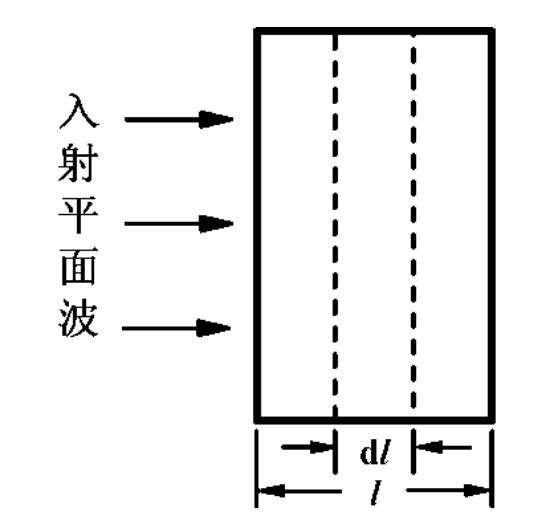
\includegraphics[width=0.2\textwidth]{均匀介质.png}
							\caption{均匀媒质对光的吸收}
							\label{fig:graph6}
						\end{figure}
						
					\item \textbf{比尔定律}:\\
					比尔定律(Beer's law),也称为比尔-朗伯定律(Beer-Lambert law),是描述光线透过吸收性均匀介质时光强衰减规律的定律,是朗伯定律的一个特例。比尔定律的数学形式为:
					\[ A = \alpha c l \]
					$A$表示吸光度,$\alpha$是摩尔吸光系数,$c$为浓度,$l$是光通过溶液的路径长度。
					在比尔定律成立时,就可用测量吸收的方法来测定物质的浓度。这就是快速测定物质浓度的吸收光谱分析法。
						
						\begin{figure}[H]
							\centering
							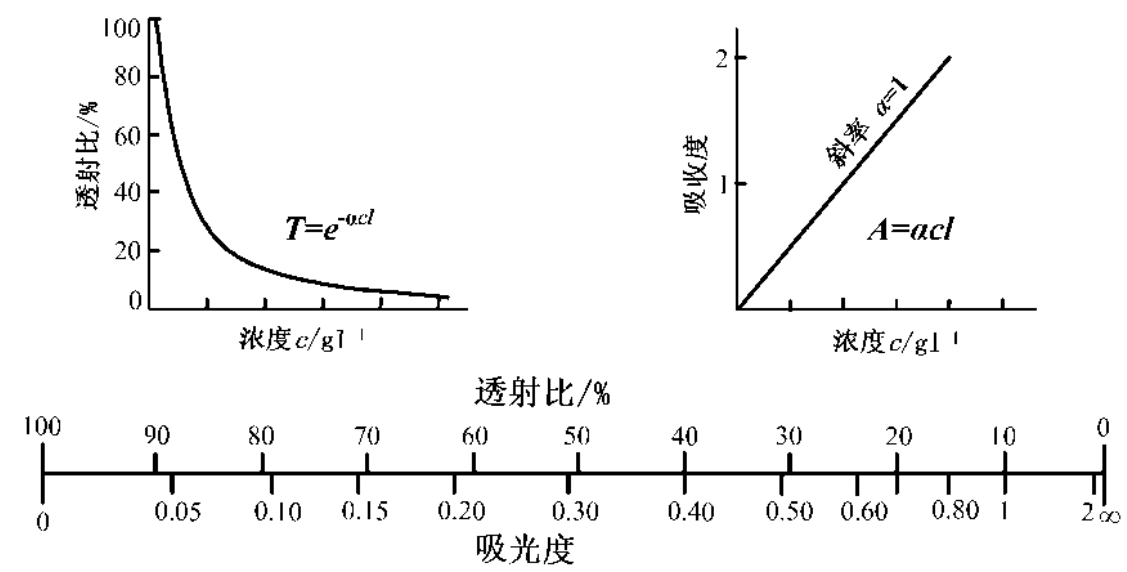
\includegraphics[width=0.6\textwidth]{比尔图像.png}
							\caption{比尔定律示意图和吸收度、投射比标度的比较}
							\label{fig:graph7}
						\end{figure}
	%				\item 光谱仪和光学多通道分析仪:
						
					
				\end{enumerate}
			
		\end{enumerate}
	
	
	\subsection{实验前思考题}
		%思考题1
		\begin{question}
			日常生活中,光源可以分为热光源和冷光源,请分别说明太阳光、蜡烛、白炽灯、荧光灯、 LED 灯等属于哪一类光源,为什么?
		\end{question}
		
		在日常生活中,光源通常可以分为热光源和冷光源两类,具体如下:

\begin{enumerate}[label=\arabic*.]
    \item \textbf{热光源}:热光源是指其发光是由高温物质的热辐射产生的光线。这种光源通常是通过加热固体、液体或气体至非常高的温度来产生的。热光源的光谱通常是连续的,包含了各种波长的光线。太阳是典型的热光源,因为它的光是由太阳表面高温引起的热辐射所产生的。
    
    \item \textbf{冷光源}:冷光源是指其发光不是由高温物质的热辐射产生的,而是通过其他方式产生的光线,例如电击激发或化学反应等。冷光源的光谱通常是不连续的,具有明显的发射线。常见的冷光源包括荧光灯和 LED 灯等。
\end{enumerate}
综上所述,太阳光、蜡烛和白炽灯属于热光源,而荧光灯和 LED 灯属于冷光源。
	
	
	% 实验记录	
	\clearpage
	
	% 顶栏
	\begin{table}
		\renewcommand\arraystretch{1.7}
		\centering
		\begin{tabularx}{\textwidth}{|X|X|X|X|}
			\hline
			专业: & 物理学 & 年级: & 2022级 \\
			\hline
			姓名: &  黄罗琳& 学号: & 22344001\\
			\hline
			室温: &26℃  & 实验地点: & A522 \\
			\hline
			学生签名:&  
\includegraphics[width=1cm]{签字.jpg} & 评分: &\\
			\hline
			实验时间:& 2024/4/18 & 教师签名:&\\
			\hline
		\end{tabularx}
	\end{table}
	% ---
	
	% 小标题
	\section{ETX 实验名称×××  \quad\heiti 实验记录}
	% ---
	
	% 实验过程记录
	\subsection{实验内容、步骤与结果}
	
	%
	\subsubsection{原子发射光谱的观测}
	\begin{enumerate}
		\item 拍摄钠灯光谱
		\begin{enumerate}
			\item 选择合适的积分次数和积分时间。实际实验中选择了“积分时间150ms,积分次数50次”
			
			\item 将光纤一端连接光谱仪,一端关闭,测量暗噪声。 
			
			\item 将光纤另一端装上支架,将支架对准未开启NA灯的环境,测量环境噪声。
			
			\item 选用S-d模式,将暗噪声与环境噪声都扣除后,将支架对准钠灯,测量钠灯光谱。
			
		\end{enumerate}
        软件给出如下实验图像,放大后经过寻峰后得出钠双黄线\\
		测得波长值分别为$\lambda_1=588.72nm$和$\lambda_2=589.34nm$
		\begin{figure}[!htb]
			\centering
			\begin{minipage}{0.35\textwidth}
				\centering
				\includegraphics[width=\linewidth]{钠.JPG}
				
				\label{fig:sodium_spectrum}
			\end{minipage}%
			\hspace{0.1\textwidth}
			\begin{minipage}{0.35\textwidth}
				\centering
				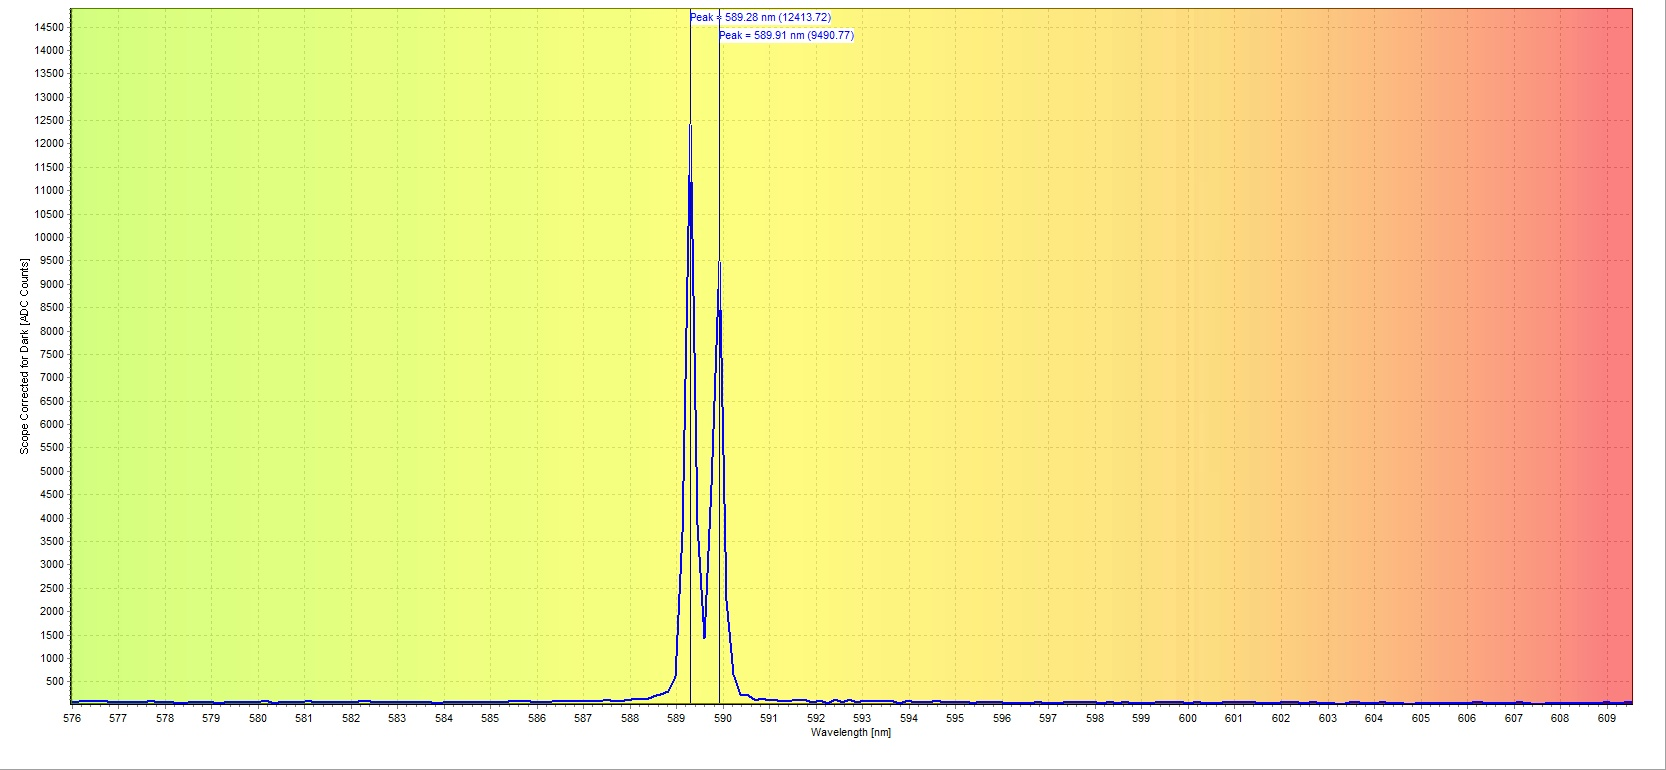
\includegraphics[width=\linewidth]{钠双黄线.JPG}
				
				\label{fig:sodium_double_yellow_lines}
			\end{minipage}
			\caption{钠的光谱图像}
			\label{fig:sodium_spectra}
		\end{figure}
		\item \textbf{拍摄汞灯光谱}
		重复实验步骤,测量汞灯光谱。
		\begin{figure}[H]
			\centering
			\begin{minipage}{0.35\textwidth}
				\centering
				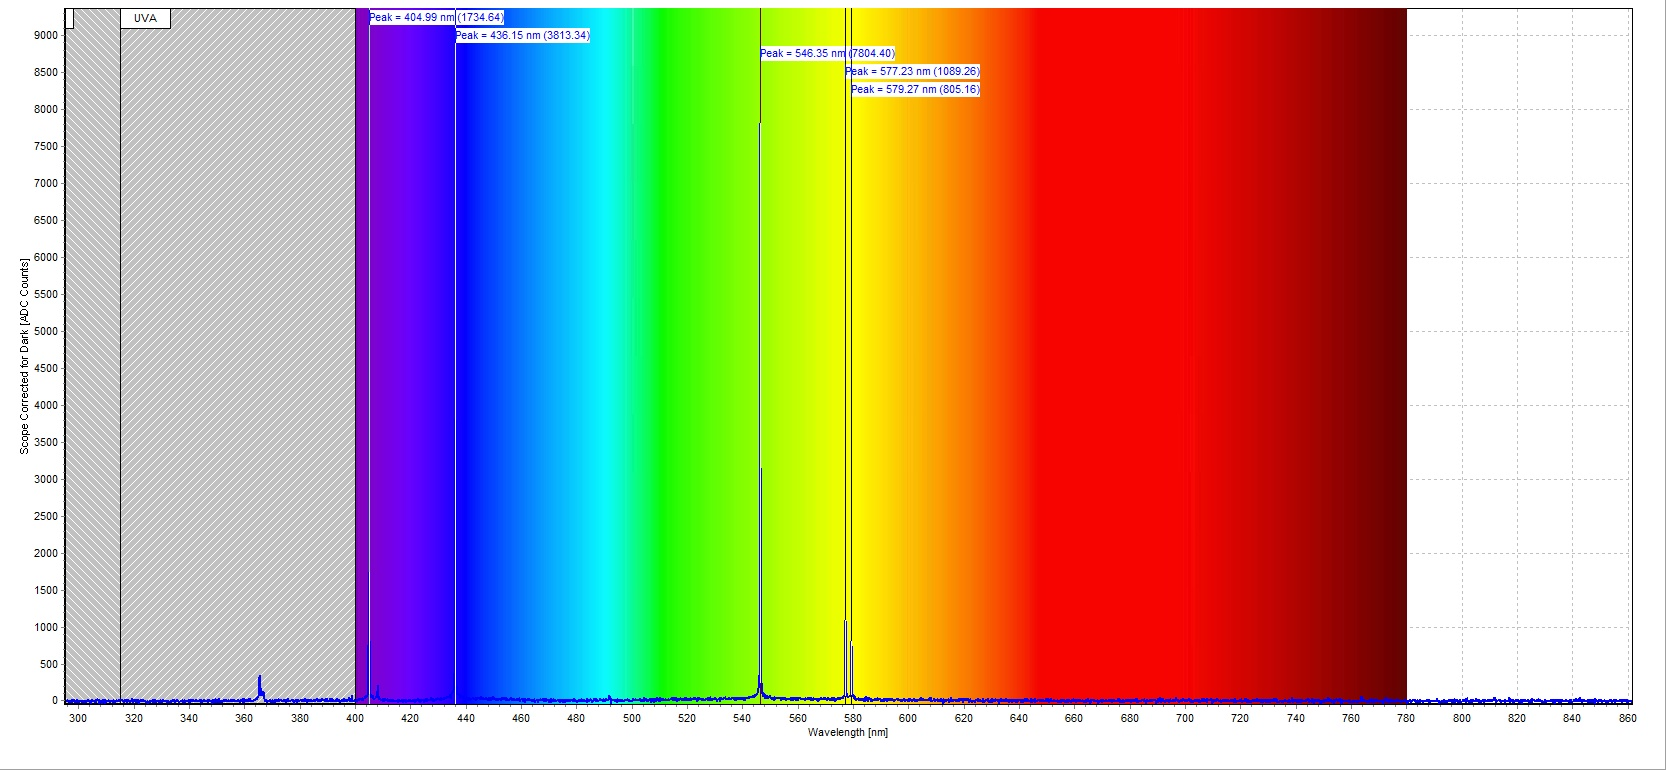
\includegraphics[width=\linewidth]{汞灯.JPG}
			
				\label{fig:mercury_lamp1}
			\end{minipage}%
			\hspace{0.1\textwidth}
			\begin{minipage}{0.35\textwidth}
				\centering
				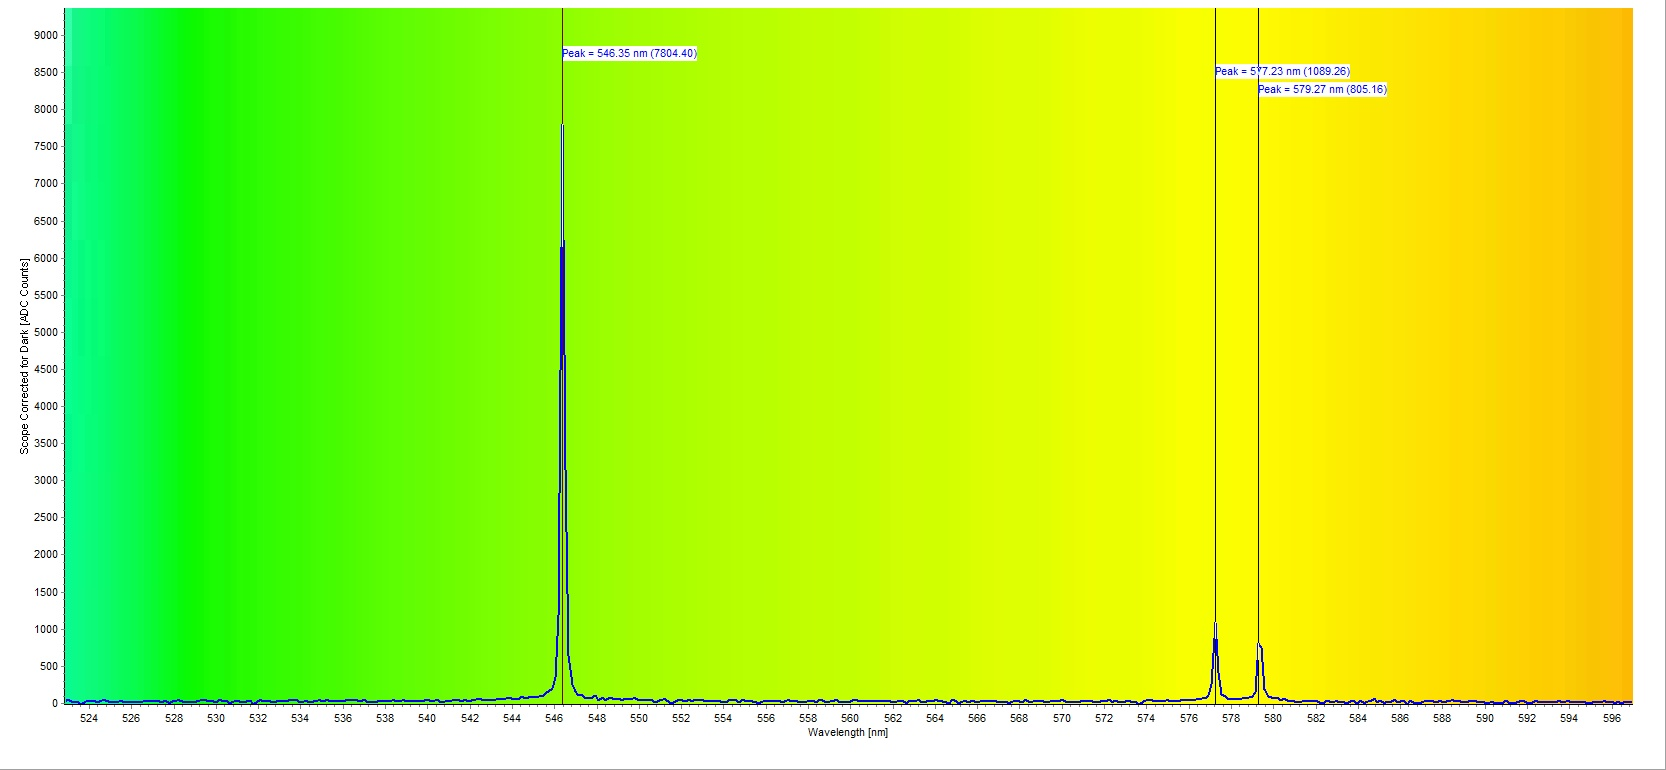
\includegraphics[width=\linewidth]{汞灯2.JPG}
				
				\label{fig:mercury_lamp2}
			\end{minipage}
		 \caption{汞灯的图像2}
			\label{fig:mercury_lamps}
		\end{figure}
		根据实验图像,可得545.90nm,435.59nm,404.41nm,578.85nm和576.65nm的谱线,最高峰是545.90nm
	\end{enumerate}	

	%
	\subsubsection{}
	\begin{enumerate}
		\item \begin{table}[h]
			\centering
			\caption{表格示例}
			\label{tab:tab1}
			\begin{tabular}{|c|c|c|c|c|c|}
				\hline
				组1/序号i & 1 & 2 & 3 & 4 & 5 \\
				$v_{1i}(m/s)$ & 1.26 & 1.08 & 1.00 & 0.75 & 0.38 \\
				$f_{1i}(Hz)$ & 40073 & 40127 & 40105 & 40088 & 40066 \\
				\hline
				组2/序号i & 1 & 2 & 3 & 4 & 5 \\
				$v_{2i}(m/s)$ & 1.21 & 1.06 & 0.99 & 0.52 & 0.57 \\
				$f_{2i}(Hz)$ & 40143 & 40125 & 40084 & 40080 & 40067 \\
				\hline
				组3/序号i & 1 & 2 & 3 & 4 & 5 \\
				$v_{3i}(m/s)$ & 1.15 & 0.98 & 0.78 & 0.59 & 0.36 \\
				$f_{3i}(Hz)$ & 40135 & 40115 & 40092 & 40070 & 40044 \\
				\hline
			\end{tabular}
		\end{table}		
	\end{enumerate}
	
	% ---
	
	% 原始数据
	\clearpage
	\subsection{原始数据记录}
	实验记录本上的原始数据见%\cref{}(签字)。
	
	实验台桌面整理见%\textbf{附件}部分(\cref{})。
	
	其它原始数据见%\cref{}。
	% ---
	
	% 问题记录
	\subsection{实验过程遇到问题及解决办法}
	\begin{enumerate}
		\item 
	\end{enumerate}
	% ---
	
	
	
	% 分析与讨论	
	\clearpage
	
	% 顶栏
	\begin{table}
		\renewcommand\arraystretch{1.7}
		\begin{tabularx}{\textwidth}{|X|X|X|X|}
			\hline
			专业:& 物理学 &年级:& 2022级\\
			\hline
			姓名: &  & 学号:& \\
			\hline
			日期:&  & 评分: &\\
			\hline
		\end{tabularx}
	\end{table}
	% ---
	
	% 小标题
	\section{ETX 实验名称××× \quad\heiti 分析与讨论}
	% ---
	
	% 数据处理
	\subsection{实验数据分析}
	
	%
	\subsubsection{}
	\begin{enumerate}
		\item 
	\end{enumerate}
	
	%
	\subsubsection{}
	\begin{enumerate}
		\item 
	\end{enumerate}
	
	%
	\subsubsection{}
	
	% ---
	
	% 实验后思考题
	\subsection{实验后思考题}
	
	%思考题1
	\begin{question}
		
	\end{question}
	
	% 思考题2
	\begin{question}
		
	\end{question}
	
	% 思考题3
	\begin{question}
		
	\end{question}
	
	% ---
	
	
	% 结语部分
	\clearpage
	
	% 小标题
	\section{ETX 实验名称××× \quad\heiti 结语}
	% ---
	
	% 总结、杂谈与致谢
	\subsection{实验心得和体会、意见建议等}
	\begin{enumerate}
		\item 
	\end{enumerate}
	% ---
	

	% 附件
	\subsection{附件及实验相关的软硬件资料等}
	试验台桌面整理如%\cref{}所示。
	
	实验报告个人签名如

	% ---
	
	
\end{document}